% Enzyme Discovery Agent — progress-report deck
% Build:  pdflatex progress_report.tex  (run twice)
\documentclass[aspectratio=169,11pt]{beamer}

\usepackage[T1]{fontenc}
\usepackage[utf8]{inputenc}
\usepackage{helvet}
\renewcommand{\familydefault}{\sfdefault}
\usepackage{graphicx}
\usepackage{tikz}
\usetikzlibrary{arrows.meta,positioning}
\usepackage{xcolor}
\usepackage{booktabs}

\definecolor{ink}{HTML}{0F172A}
\definecolor{muted}{HTML}{475569}
\definecolor{brand}{HTML}{4338CA}
\definecolor{brand2}{HTML}{0D9488}
\definecolor{accent}{HTML}{E11D48}
\definecolor{soft}{HTML}{EEF2FF}
\definecolor{rule}{HTML}{CBD5E1}
\definecolor{good}{HTML}{15803D}

\usecolortheme{default}
\setbeamercolor{normal text}{fg=ink}
\setbeamercolor{frametitle}{fg=brand}
\setbeamercolor{itemize item}{fg=brand2}
\setbeamercolor{itemize subitem}{fg=brand2}
\setbeamerfont{frametitle}{series=\bfseries,size=\LARGE}
\setbeamertemplate{navigation symbols}{}
\setbeamertemplate{itemize item}{\small\raise0.5pt\hbox{\textbullet}}
\setbeamertemplate{itemize subitem}{\scriptsize\raise0.5pt\hbox{--}}
\setbeamertemplate{frametitle}{%
  \vspace*{0.6em}\hspace*{0.2em}%
  {\usebeamerfont{frametitle}\usebeamercolor[fg]{frametitle}\insertframetitle}\\[-0.2em]
  {\color{rule}\rule{\dimexpr\paperwidth-1.2em\relax}{1.2pt}}\vspace*{-0.2em}}
\setbeamertemplate{footline}{%
  \hbox{}\hfill{\color{muted}\scriptsize Enzyme Discovery Agent — progress\quad\insertframenumber\ /\ \inserttotalframenumber\ }\vspace*{0.5em}}

\newcommand{\hl}[1]{{\color{brand}\textbf{#1}}}
\newcommand{\hlt}[1]{{\color{brand2}\textbf{#1}}}
\newcommand{\hla}[1]{{\color{accent}\textbf{#1}}}
\newcommand{\gd}[1]{{\color{good}\textbf{#1}}}
\newcommand{\chip}[2]{\tikz[baseline=(x.base)]{\node[fill=#1!12,draw=#1,rounded corners=3pt,inner sep=3pt,text=#1!75!black,font=\footnotesize\bfseries](x){#2};}}

\begin{document}

% ---------- Title ----------
{\setbeamertemplate{footline}{}
\begin{frame}[plain]
  \vspace*{1.4em}
  {\color{brand}\rule{\textwidth}{2pt}}\\[1.2em]
  {\Huge\bfseries\color{ink} Enzyme Discovery Agent}\\[0.5em]
  {\LARGE\color{muted} Progress report — what we changed, and how it validated}\\[1.4em]
  \chip{brand2}{better discovery}\quad
  \chip{brand}{cheaper \& cleaner}\quad
  \chip{good}{validated on the benchmark}\\[1.2em]
  {\color{brand}\rule{\textwidth}{2pt}}
\end{frame}}

% ---------- TL;DR ----------
\begin{frame}{The short version}
  On our benchmark (find enzymes that join a diacid and a diamine — nylon-6,6
  precursors):
  \vspace{0.6em}
  \begin{itemize}
    \item the candidate that was \hla{wrongly ranked \#1} — an aromatic amino-acid
      conjugator — now \gd{drops out of the list entirely}
    \item a genuine diamine ligase (\hlt{PuuA}) is now \gd{\#1}, and the exact answer
      (\hlt{DdaG}) moved up to \gd{\#3}
    \item the analogues we were missing (\hlt{DesD, AsbA, AsbB, \dots}) are now \gd{all found}
    \item and it got \gd{cheaper} (\textasciitilde 2.18M \textrightarrow{} \textasciitilde 1.43M tokens)
      with \gd{no slowdown} (\textasciitilde 32 min)
  \end{itemize}
  \vspace{0.4em}
  {\footnotesize\color{muted} Every change ships with the tests passing and the answer
  still hidden from the agent.}
\end{frame}

% ---------- Context ----------
\begin{frame}{One line of context}
  \vspace{0.5em}
  \begin{center}
    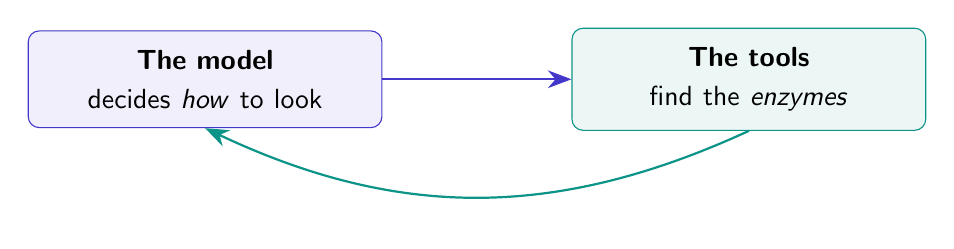
\begin{tikzpicture}[every node/.style={font=\small},node distance=24mm]
      \node[draw=brand,fill=brand!8,rounded corners,text width=4cm,align=center,inner sep=7pt,font=\bfseries]
        (llm) {The model\\[2pt]\normalfont decides \emph{how} to look};
      \node[right=of llm,draw=brand2,fill=brand2!8,rounded corners,text width=4cm,align=center,inner sep=7pt,font=\bfseries]
        (tools) {The tools\\[2pt]\normalfont find the \emph{enzymes}};
      \draw[-{Stealth[length=3mm]},thick,brand] (llm)--(tools);
      \draw[-{Stealth[length=3mm]},thick,brand2] (tools.south) to[bend left=25] (llm.south);
    \end{tikzpicture}
  \end{center}
  \vspace{0.6em}
  \begin{center}\small
  The agent discovers enzymes for a target reaction \hla{without ever being told the
  answer}. The work below makes that discovery \hl{more complete}, its ranking
  \hl{more honest}, and the whole thing \hl{cheaper}.
  \end{center}
\end{frame}

% ---------- Changes: discovery ----------
\begin{frame}{What we changed — finding better enzymes}
  \begin{itemize}
    \item \hlt{Honest substrate matching.} When the target has two substrates, each of
      the enzyme's natives can now serve only \emph{one} of them — so a candidate can't
      look good by matching both onto its single best native. \emph{(This is what fixed
      the wrong \#1.)}
    \item \hlt{Keep every enzyme that fits.} We used to keep only a family's best two
      members; now we keep every member that runs the right direction and has a real
      substrate to compare. \emph{(This recovered the missing analogues.)}
    \item \hlt{Actually evaluate all of them.} Evaluation is just database lookups, so
      looking at more is basically free — we now check every candidate, in parallel,
      instead of stopping at a budget.
    \item \hlt{Read literature more sharply.} Instead of bulk-reading dozens of papers,
      we read a few and keep only the enzymes they \emph{name} — the one thing
      literature uniquely gives us (it's how we reach the answer's own gene cluster).
  \end{itemize}
\end{frame}

% ---------- Changes: efficiency + cleanup ----------
\begin{frame}{What we changed — cheaper, and cleaner underneath}
  \begin{columns}[T]
    \begin{column}{0.5\textwidth}
      \hl{Cheaper \& no slower}
      \begin{itemize}
        \item much lighter literature reading (\textasciitilde 90\% fewer model calls,
          no stalling on paywalls)
        \item evaluate candidates in parallel
        \item \gd{\textasciitilde 2.18M \textrightarrow{} \textasciitilde 1.43M tokens} per run
      \end{itemize}
    \end{column}
    \begin{column}{0.5\textwidth}
      \hla{Cleaner code}
      \begin{itemize}
        \item folded nine control gates into one clean pipeline
        \item removed duplicated scoring / direction logic
        \item deleted \textasciitilde 730 lines that weren't doing anything
      \end{itemize}
      \vspace{0.4em}
      \begin{center}\chip{brand2}{all tests pass}\quad\chip{brand}{answer still hidden}\end{center}
    \end{column}
  \end{columns}
  \vspace{0.8em}
  \begin{center}\small\color{muted}
    None of the cleanup changes behavior — it just makes the pipeline easier to work on.
  \end{center}
\end{frame}

% ---------- Validation ----------
\begin{frame}{Did it work? — before vs after}
  \vspace{0.6em}
  \begin{center}
  \renewcommand{\arraystretch}{1.4}
  \resizebox{0.98\textwidth}{!}{%
  \begin{tabular}{lcc}
    \toprule
     & \textbf{Before} & \textbf{After} \\
    \midrule
    The wrongly-ranked \#1 (an aromatic conjugator) & \hla{\#1} & \gd{not ranked} \\
    So the \#1 candidate is now\dots               & aromatic conjugator & \gd{PuuA (a real diamine ligase)} \\
    DdaG, the exact answer                          & \#4 & \gd{\#3} \\
    Missing analogues (DesD, AsbA, AsbB, \dots)     & mostly absent & \gd{all recovered} \\
    Tokens per run                                  & \textasciitilde 2.18M & \gd{\textasciitilde 1.43M} \\
    Wall-clock                                      & \textasciitilde 32 min & \textasciitilde 32 min \\
    \bottomrule
  \end{tabular}}
  \end{center}
  \vspace{0.7em}
  {\footnotesize\color{muted} Ground truth is used only to grade the run afterwards —
  never given to the agent.}
\end{frame}

% ---------- The concrete fix ----------
\begin{frame}{Why the old \#1 was wrong — and how it's fixed}
  \begin{columns}[T]
    \begin{column}{0.52\textwidth}
      The old \#1 was an enzyme that joins \emph{indole-acetate} to \emph{lysine}. Its
      lysine is a loose stand-in for one target substrate — and the old code let
      \hla{both} of our target substrates match onto that same lysine, so it looked far
      better than it is.\\[0.7em]
      With \hlt{one-to-one} matching, the second target substrate is forced onto the
      enzyme's \emph{other} native — an aromatic indole-acetate, nothing like a diamine
      — so its score drops to essentially \gd{zero}, and it falls out of the list.
    \end{column}
    \begin{column}{0.48\textwidth}
      \centering
      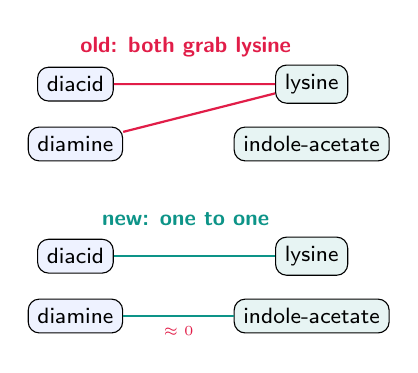
\begin{tikzpicture}[every node/.style={font=\footnotesize},yscale=0.95]
        \node[text=accent,font=\footnotesize\bfseries] at (1.4,2.5) {old: both grab lysine};
        \node[draw,rounded corners,fill=soft] (t1) at (0,2) {diacid};
        \node[draw,rounded corners,fill=soft] (t2) at (0,1.2) {diamine};
        \node[draw,rounded corners,fill=brand2!10] (n1) at (3.0,2) {lysine};
        \node[draw,rounded corners,fill=brand2!10] (n2) at (3.0,1.2) {indole-acetate};
        \draw[accent,thick] (t1)--(n1);
        \draw[accent,thick] (t2)--(n1);
        \node[text=brand2,font=\footnotesize\bfseries] at (1.4,0.2) {new: one to one};
        \node[draw,rounded corners,fill=soft] (u1) at (0,-0.3) {diacid};
        \node[draw,rounded corners,fill=soft] (u2) at (0,-1.1) {diamine};
        \node[draw,rounded corners,fill=brand2!10] (m1) at (3.0,-0.3) {lysine};
        \node[draw,rounded corners,fill=brand2!10] (m2) at (3.0,-1.1) {indole-acetate};
        \draw[brand2,thick] (u1)--(m1);
        \draw[brand2,thick] (u2)--(m2) node[midway,below,font=\tiny,text=accent]{$\approx 0$};
      \end{tikzpicture}
    \end{column}
  \end{columns}
\end{frame}

% ---------- Next ----------
\begin{frame}{What's still rough — next steps}
  \begin{itemize}
    \item \hl{Literature recall.} We still miss some of the field's best papers because
      we search with the wrong words (and a few are paywalled). Rewriting queries helps,
      but not reliably yet.
    \item \hl{Matching a family to its fold.} A few promising families get matched to the
      wrong structural fold, so they never get a fit score and don't show up on the map —
      even when one of their members ranks well. Fixing this is the next big win.
    \item \hl{Speed.} Almost all the time is the model reading long prompts; the wins are
      shorter prompts and running the final steps in parallel.
    \item \hl{Ranking.} A couple of scoring measures still don't fully agree — worth
      unifying, then re-checking ranking quality run over run.
  \end{itemize}
\end{frame}

% ---------- Closing ----------
{\setbeamertemplate{footline}{}
\begin{frame}[plain]
  \vspace*{2.2em}
  {\color{brand}\rule{\textwidth}{2pt}}\\[1.0em]
  {\LARGE\bfseries\color{ink} Better answers, honestly ranked, for less.}\\[0.8em]
  {\large\color{muted} The wrong \#1 is gone, the real answers rose, the missing}\\
  {\large\color{muted} analogues came back — cheaper, and still with the answer hidden.}\\[1.4em]
  \chip{brand2}{honest substrate matching}\quad
  \chip{brand}{keep everything that fits}\quad
  \chip{good}{validated}\\[1.0em]
  {\color{brand}\rule{\textwidth}{2pt}}
\end{frame}}

\end{document}
